\chapter{Hardware and Data Preprocessing}
\label{ch:Hardware}

As aforementioned, we used a MIMU (GaitWatch) and a force plate (Zebris FDM-S) to gather the raw gait data. In this chapter we will describe the employed hardware in detail. Subsequently, we will elaborate on how the necessary synchronisation of both systems was carried out.

\section{GaitWatch}

The GaitWatch device is a MIMU designed to monitor the motion of patients while attached to the body. It was developed at the Department of Neurology of the Ludwig-Maximilians University in Munich in conjunction with the Department of Signal Theory, Telematics and Communications of the University of Granada. The system is composed of a set of embedded magnetic and inertial sensors wired to a box containing a microcontroller. This microcontroller is in charge of collecting data from the embedded box sensors, as well as from the external measurement units, and storing them on a memory card. The various units are placed at the patient's thighs, shanks, arms and trunk as shown in Figure \ref{fig:GaitWatch_placement}. The components of the three different kinds of subunits are described below:

\begin{figure}
	\centering
	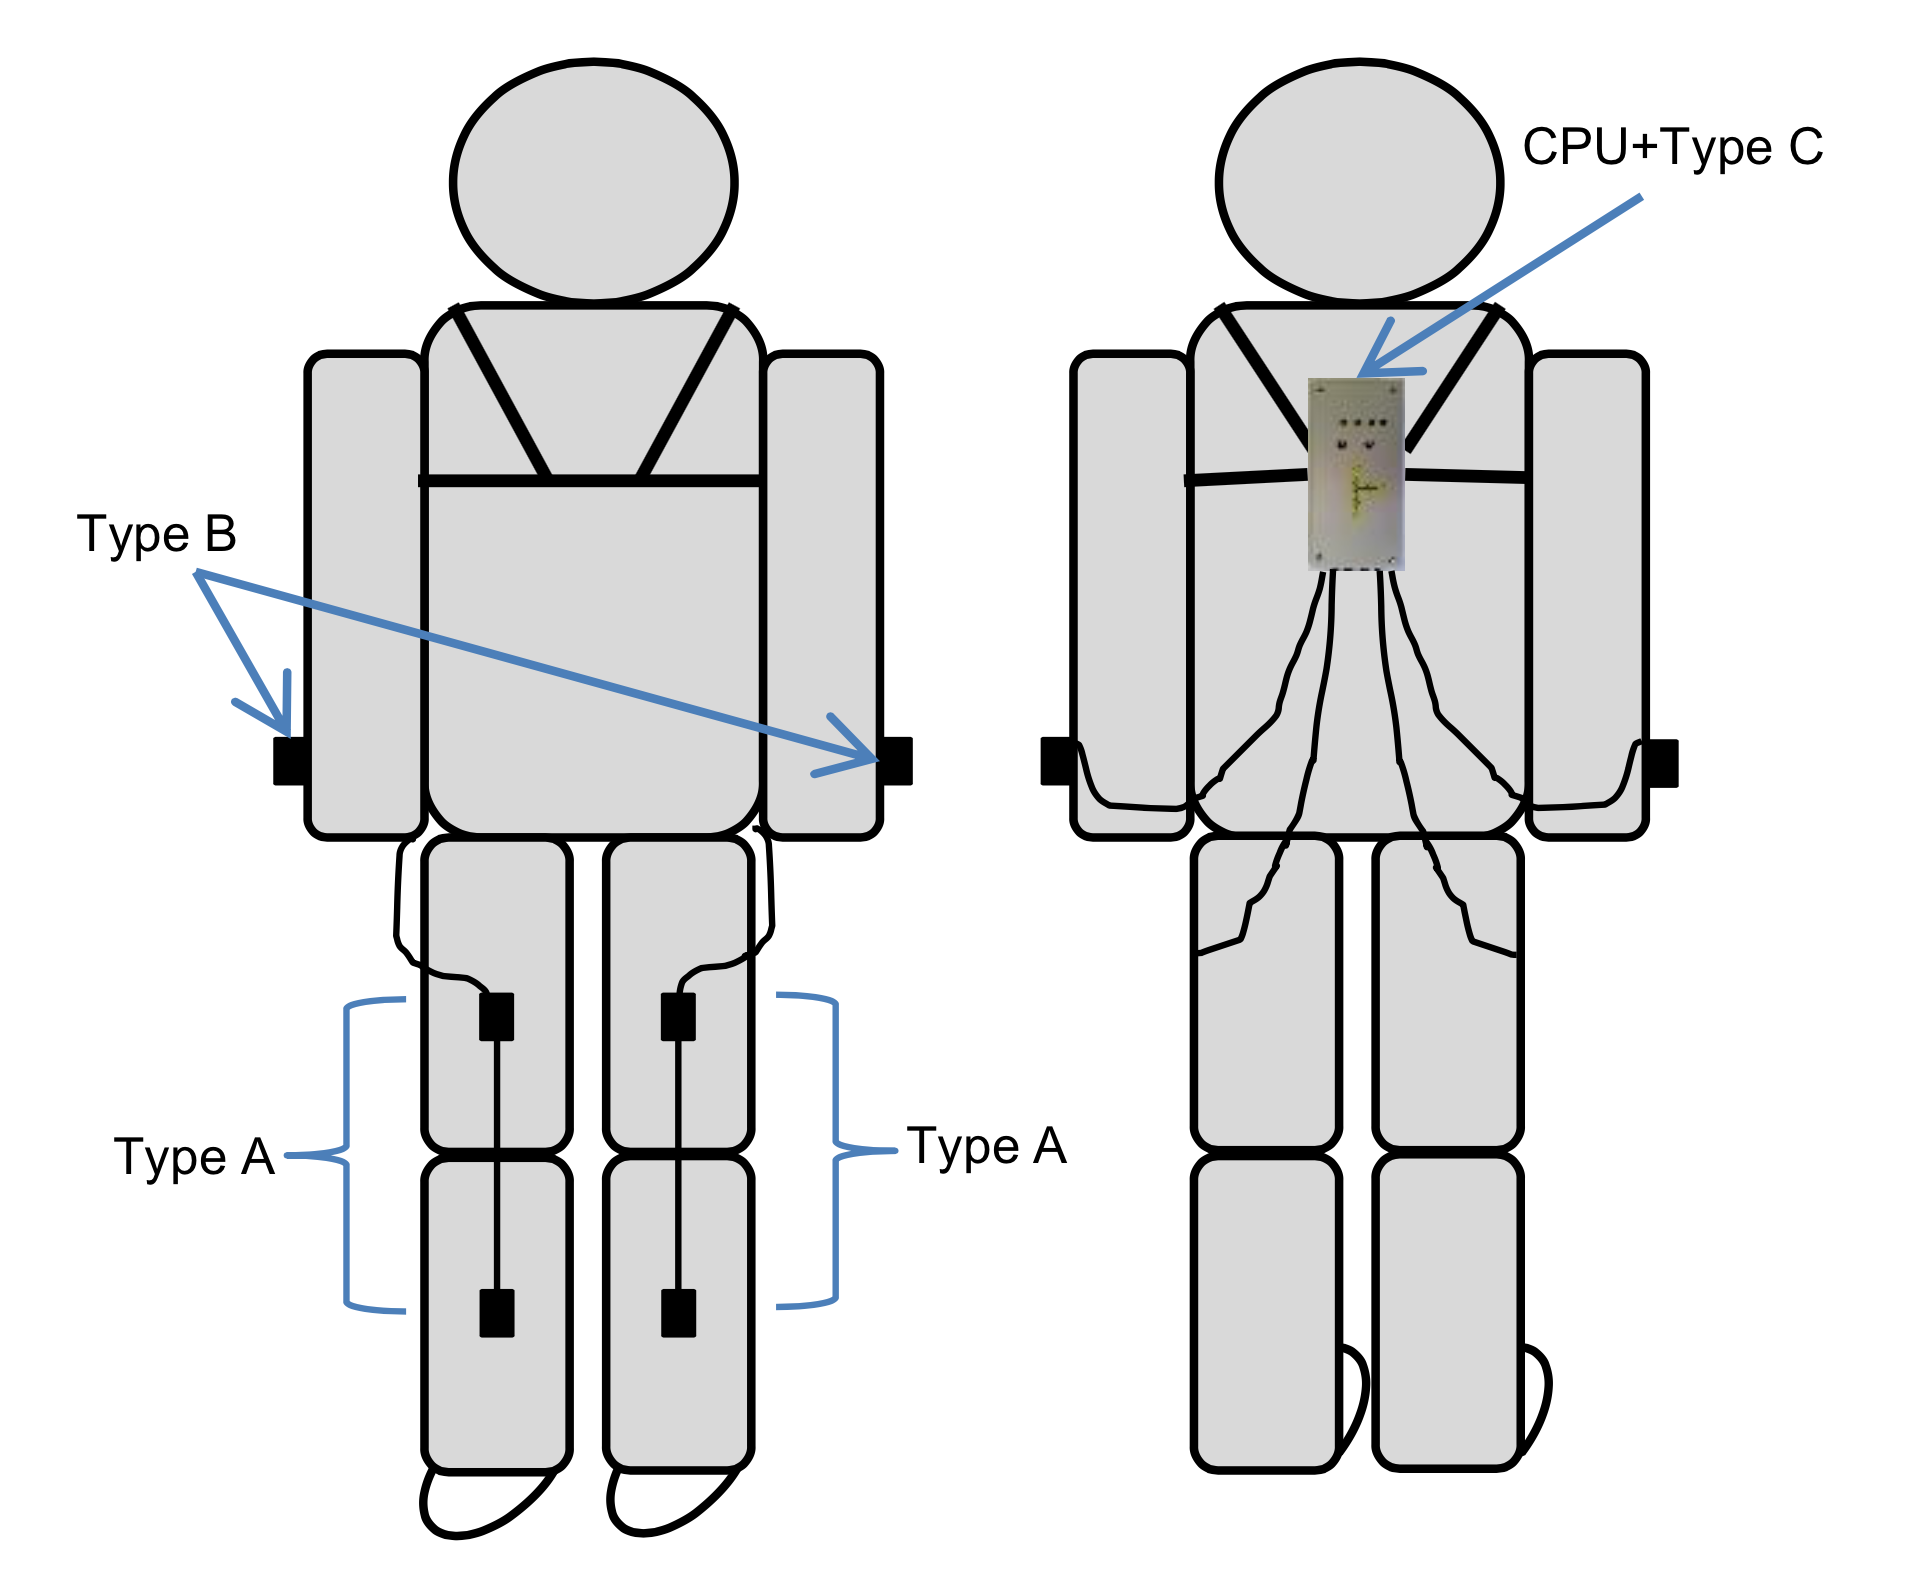
\epsfig{file=images/GaitWatch_placement, width=9cm}
	\caption{Placement of GaitWatch components at the body \cite{olivares_vicente_gaitwatch_2013}.}
	\label{fig:GaitWatch_placement}
\end{figure}

\begin{itemize}

\item \textsc{Type A} (thighs and shanks): 

IMU Analog Combo Board with 5 Degrees of Freedom \cite{IMU5} containing an IDG500 biaxial gyroscope (from which only Y axis is actually used) with a measurement range of ±500°/s \cite{IDG500} and a ±3g triaxial accelerometer, ADXL335 \cite{ADXL335}.

\item \textsc{Type B} (arms):

IDG500 biaxial gyroscope with a measurement range of ±500°/s \cite{IDG500}.

\item \textsc{Type C} (trunk):

ADXL345 triaxial accelerometer with programmable range (±2g/±4g/±8g/±16g) \cite{ADXL345},
IMU3000 triaxial gyroscope with programmable range (±250/±500/±1000/±3000°/s) \cite{IMU3000}, 
Micromag3 triaxial magnetometer with a measurement range of ±11Gauss \cite{MicroMag3}, AL-XAVRB board containing an AVR ATxmega processor \cite{AVRATxmega}.

\end{itemize}


\section{Zebris FDM-S}

The Zebris FDM-S is a force measuring plate with a sensor area of 540 x 330 mm accommodating 40 x 64 force sensors which results in 1.4 sensors per square centimetre. The data was sampled at a frequency of 120 Hz.

\section{Synchronisation}

According to the data gathering protocol in \ref{data_gathering_protocol} the raw data that was collected with the MIMU and the force plate had distinct time axes, thus a synchronisation of both systems was necessary.

In order to achieve this we created a MATLAB$\textsuperscript{\textregistered}$ routine that read the raw force plate data from separate text files, containing the data for one cycle each, carried out the calibration of the GaitWatch data and performed the synchronisation. Therefore it first detected the separate gait cycles, computed the differences between the time vectors of the force plate signals and the GaitWatch signals and corrected the force plate time vector, accordingly. Then the force plate signals were resampled at the GaitWatch sampling frequency of \mbox{200 Hz}. Eventually the whole series of signals were separated in chunks of one cycle and stored as cell array of time series objects in a .mat-file.

\begin{figure}
	\centering
	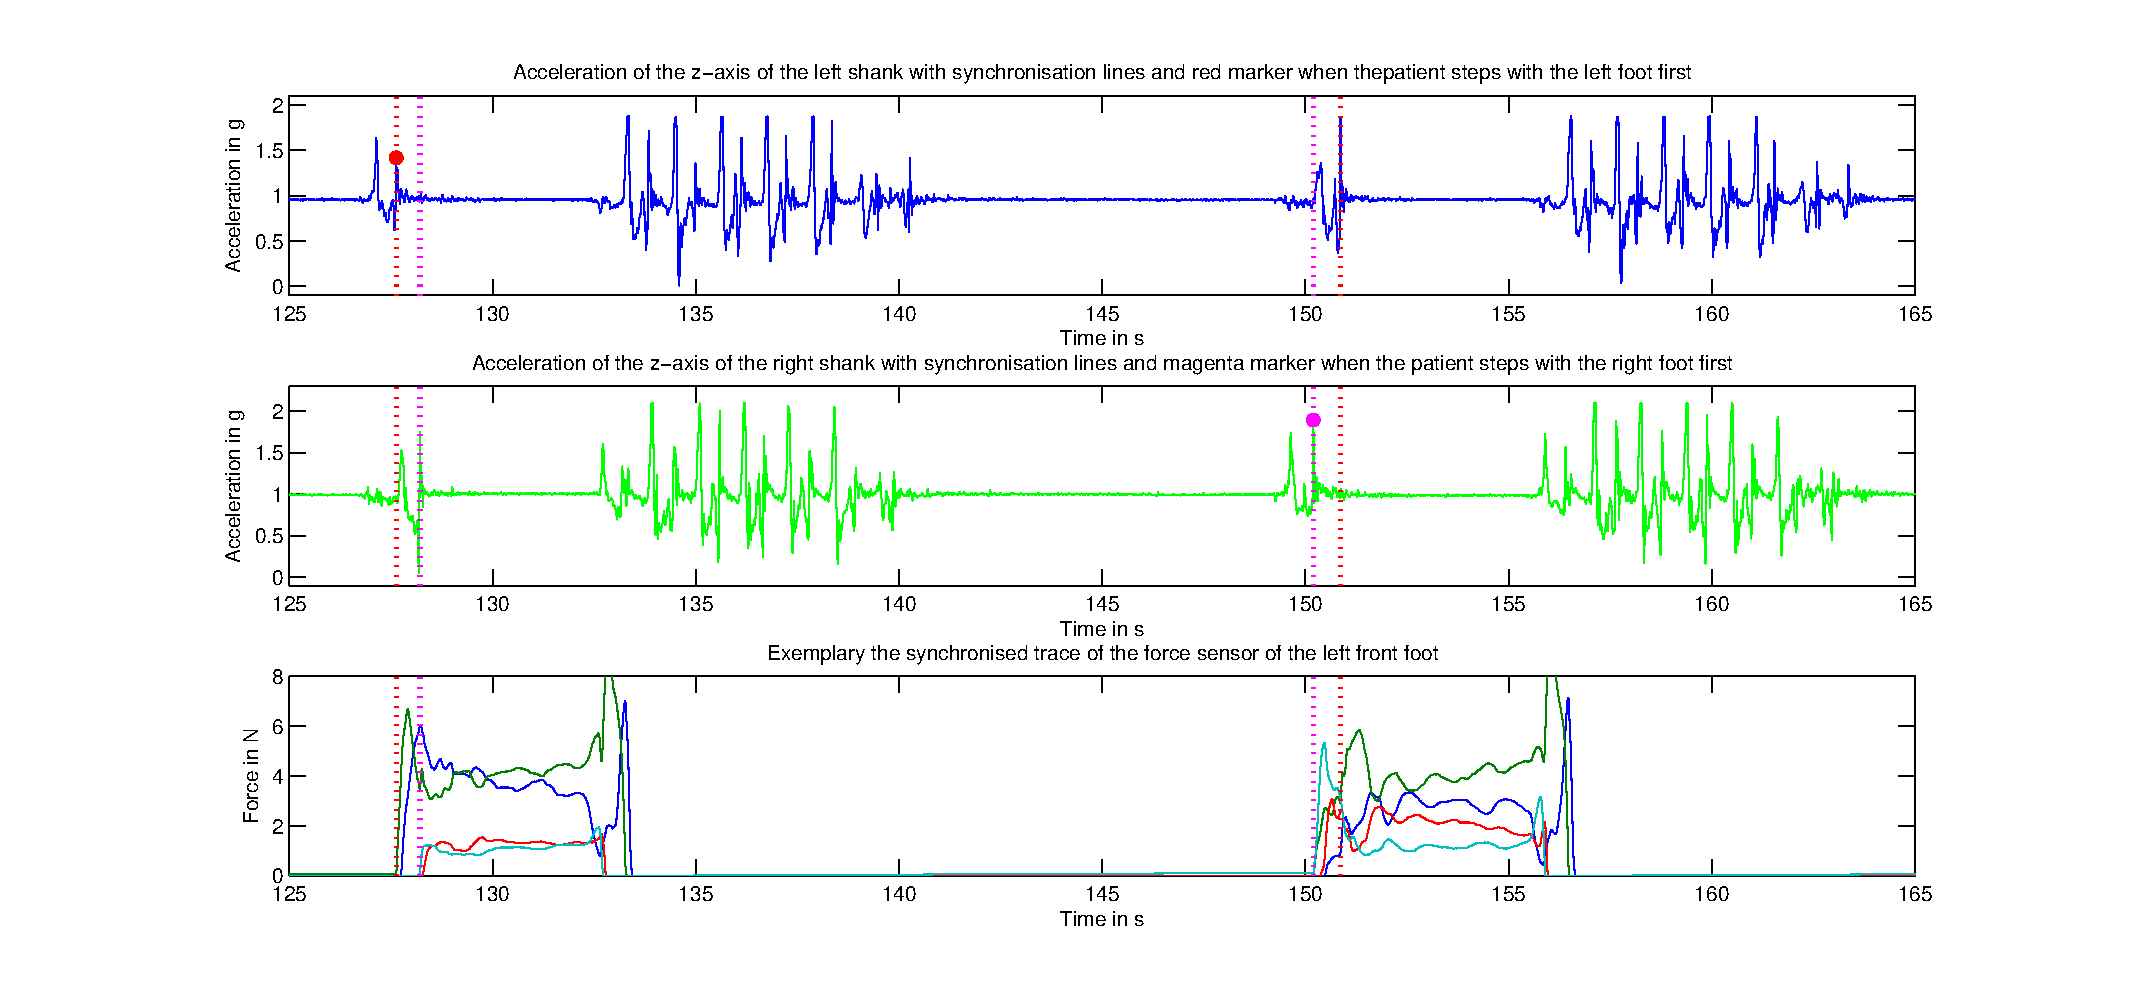
\epsfig{file=images/left_right_detect, width=16cm}
	\caption{Left-right detection}
	\label{fig:left_right_detect}
\end{figure}

Because the patient could step with a preferred limb first we added a left-right detection before we set the synchronisation points as shown in Figure \ref{fig:left_right_detect}.